%% LaTeX-Beamer template for KIT design
%% by Erik Burger, Christian Hammer
%% title picture by Klaus Krogmann
%%
%% version 2.1
%%
%% mostly compatible to KIT corporate design v2.0
%% http://intranet.kit.edu/gestaltungsrichtlinien.php
%%
%% Problems, bugs and comments to
%% burger@kit.edu

\documentclass[18pt]{beamer}

%% SLIDE FORMAT

% use 'beamerthemekit' for standard 4:3 ratio
% for widescreen slides (16:9), use 'beamerthemekitwide'
\usepackage[utf8]{inputenc}
\usepackage[T1]{fontenc}
\usepackage{templates/beamerthemekit}
%\usepackage{templates/beamerthemekitwide}

%% TITLE PICTURE

% if a custom picture is to be used on the title page, copy it into the 'logos'
% directory, in the line below, replace 'mypicture' with the 
% filename (without extension) and uncomment the following line
% (picture proportions: 63 : 20 for standard, 169 : 40 for wide
% *.eps format if you use latex+dvips+ps2pdf, 
% *.jpg/*.png/*.pdf if you use pdflatex)

\titleimage{controller}

%% TITLE LOGO

% for a custom logo on the front page, copy your file into the 'logos'
% directory, insert the filename in the line below and uncomment it

\titlelogo{ElipseLogo}

% (*.eps format if you use latex+dvips+ps2pdf,
% *.jpg/*.png/*.pdf if you use pdflatex)

%% TikZ INTEGRATION

% use these packages for PCM symbols and UML classes
% \usepackage{templates/tikzkit}
% \usepackage{templates/tikzuml}

% the presentation starts here

\title[Elipse]{Elipse -- Einteilungs Interface für das PSE}
\subtitle{Entwurfspräsentation}
\author{D. Biester, E. Dohse, P. Faller, P. Loth, L. Seufert, S. Kopmann}

\institute{IPD Snelting}

% Bibliography

\usepackage[citestyle=authoryear,bibstyle=numeric,hyperref,backend=biber]{biblatex}
\addbibresource{templates/example.bib}
\bibhang1em

\begin{document}

% change the following line to "ngerman" for German style date and logos
\selectlanguage{ngerman}

%title page
\begin{frame}
\titlepage
\end{frame}

%table of contents
%\begin{frame}{Outline/Gliederung}
%\tableofcontents
%\end{frame}

% \section{Section 1}
% %\subsection{Subsection 1.1}
% \begin{frame}{Einführung}
% \begin{itemize}
% \item PCM, Citation: \cite{becker2008a} %\language
% \pause
% \item Bullet point 2
% \item \dots
% \end{itemize}
% \end{frame}
% 
% \subsection{Subsection 1.2}
% \begin{frame}{Example slide B}
% \begin{block}{Block 1}
% \begin{itemize}
% \item Bullet point 1
% \pause
% \item Bullet point 2
% \item \dots
% \end{itemize}
% \end{block}
% \end{frame}
% 
% \section{Section 2}
% \begin{frame}{Example slide C}
% \begin{exampleblock}{Example 1}
% \begin{itemize}
% \item Bullet point 1
% \pause
% \item Bullet point 2
% \item \dots
% \end{itemize}
% \end{exampleblock}
% \end{frame}
% 
% \begin{frame}{Example slide D}
% \begin{alertblock}{Alert 1}
% \begin{itemize}
% \item Bullet point 1
% \pause
% \item Bullet point 2
% \item \dots
% \end{itemize}
% \end{alertblock}
% \end{frame}
\section{Überblick}
\begin{frame}{Überblick}
Grobentwurf:
\begin{itemize}
  \item Model-View-Controller
  \item Play-Framework
  \item ILP (Gurobi) %TODO ergänzen: einzelene Module 
\end{itemize}
\end{frame}

\begin{frame}
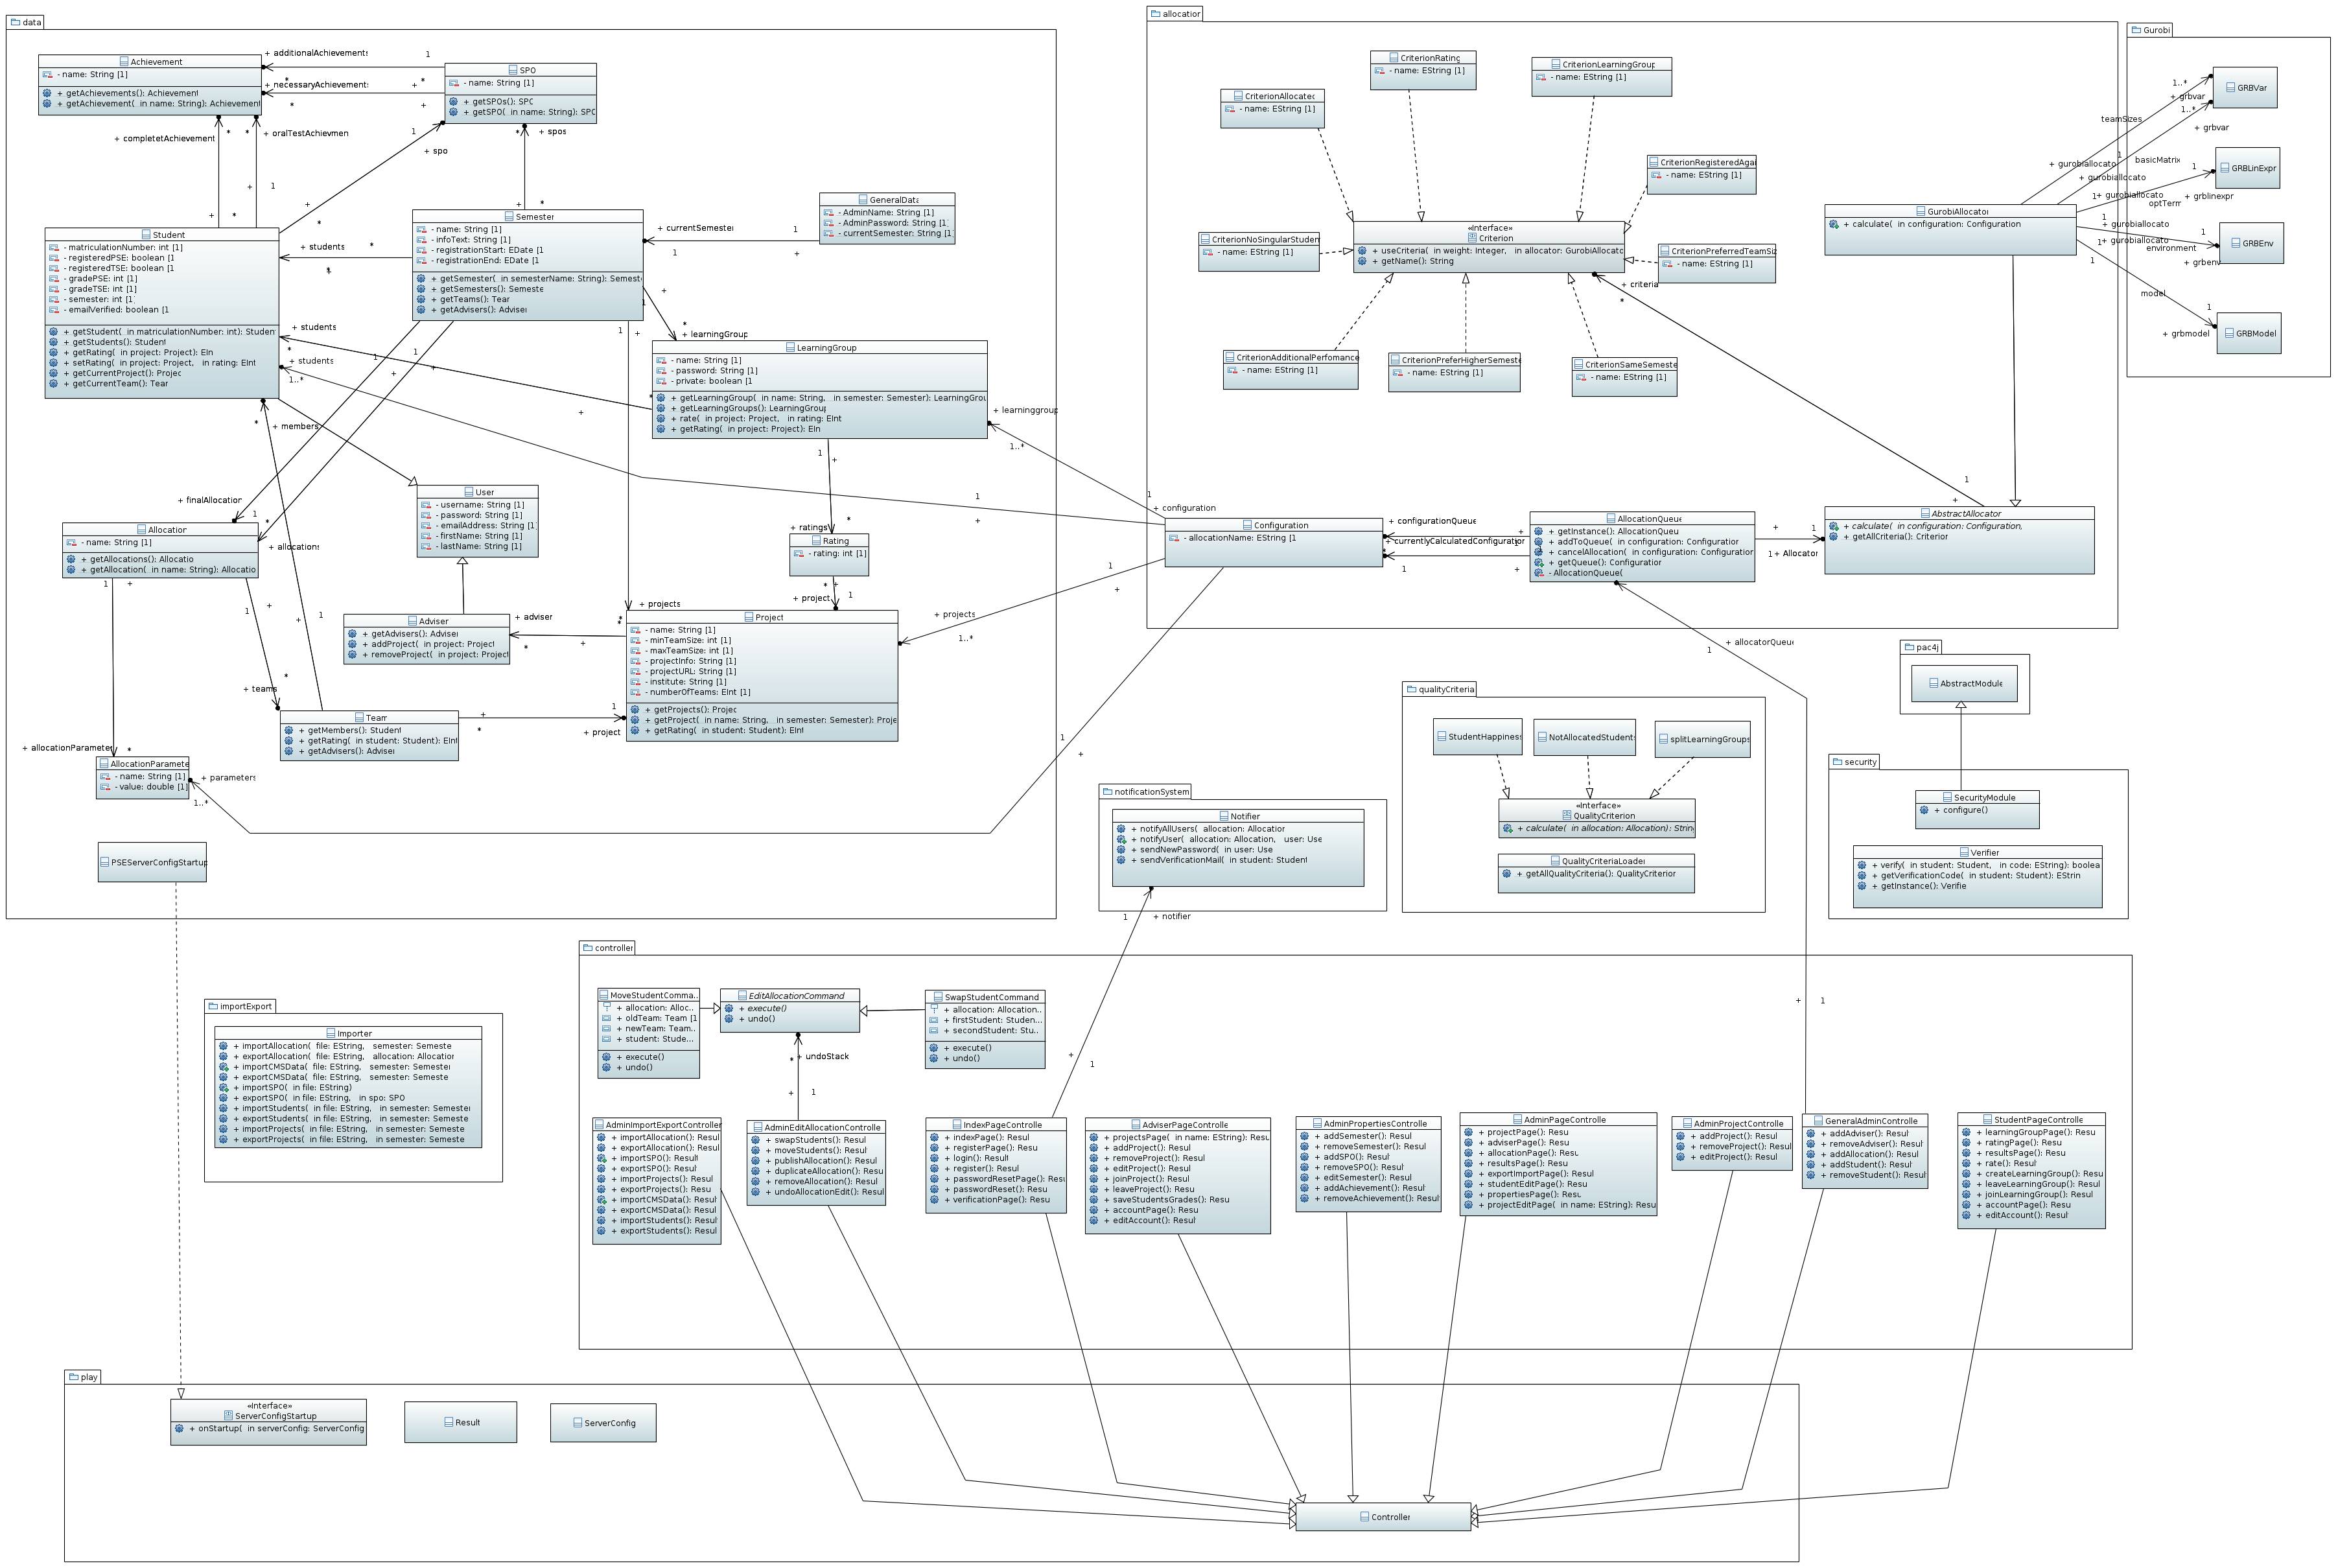
\includegraphics[width=\linewidth]{bilder/Class_Diagram.png}
\end{frame}

\subsection{Controller}
\begin{frame}{Controller}
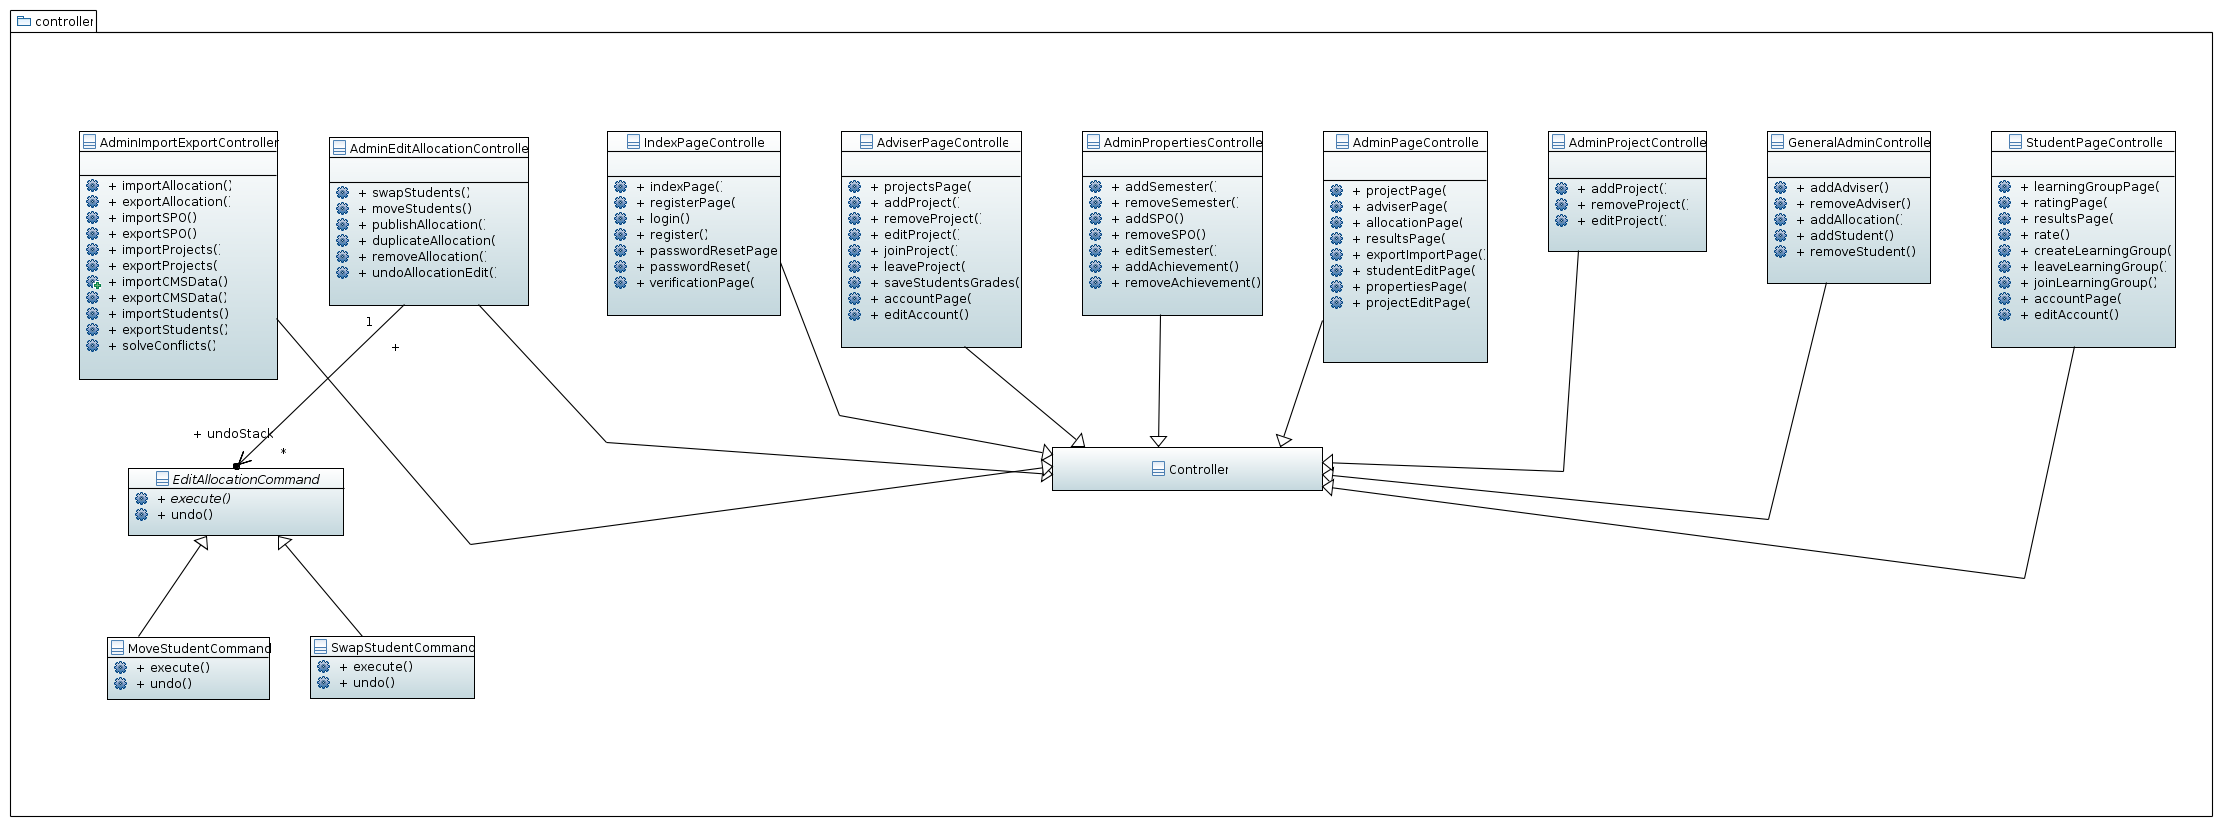
\includegraphics[width=\linewidth]{bilder/controller.png}
%TODO sollen wir controller überhaupt zeigen? wenn ja bild
\end{frame}

\subsection{Datenmodell}
\begin{frame}{Datenmodell}
% \begin{itemize}
%   \item Verwaltung über mehrere Semester
%   \item 
%TODO was noch?
% \end{itemize}
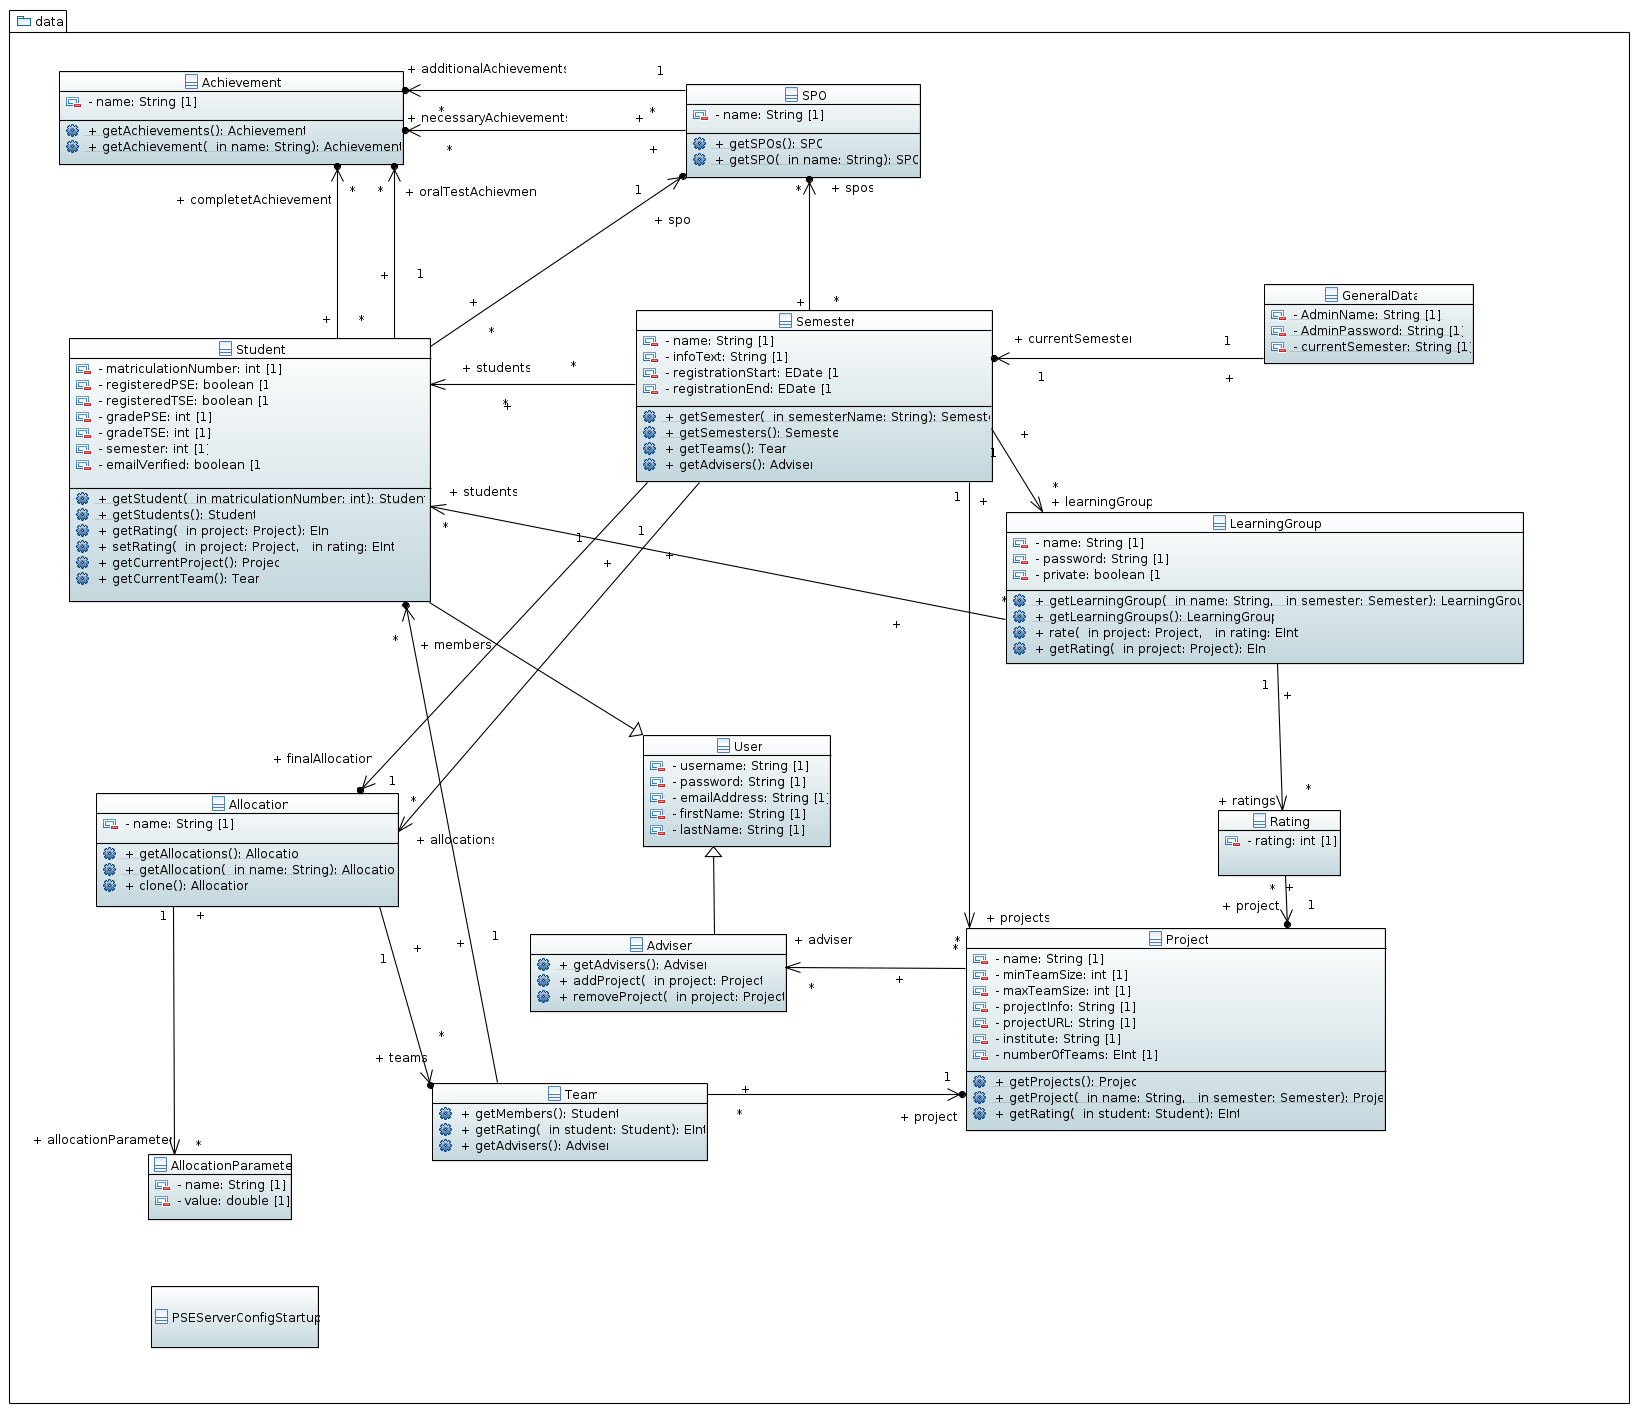
\includegraphics[width=\textheight]{bilder/daten.png}
%TODO bild 
\end{frame}

\subsection{Einteilung}
\begin{frame}{Einteilung}
% \begin{itemize}
%   \item  
%TODO was hier?
% \end{itemize}
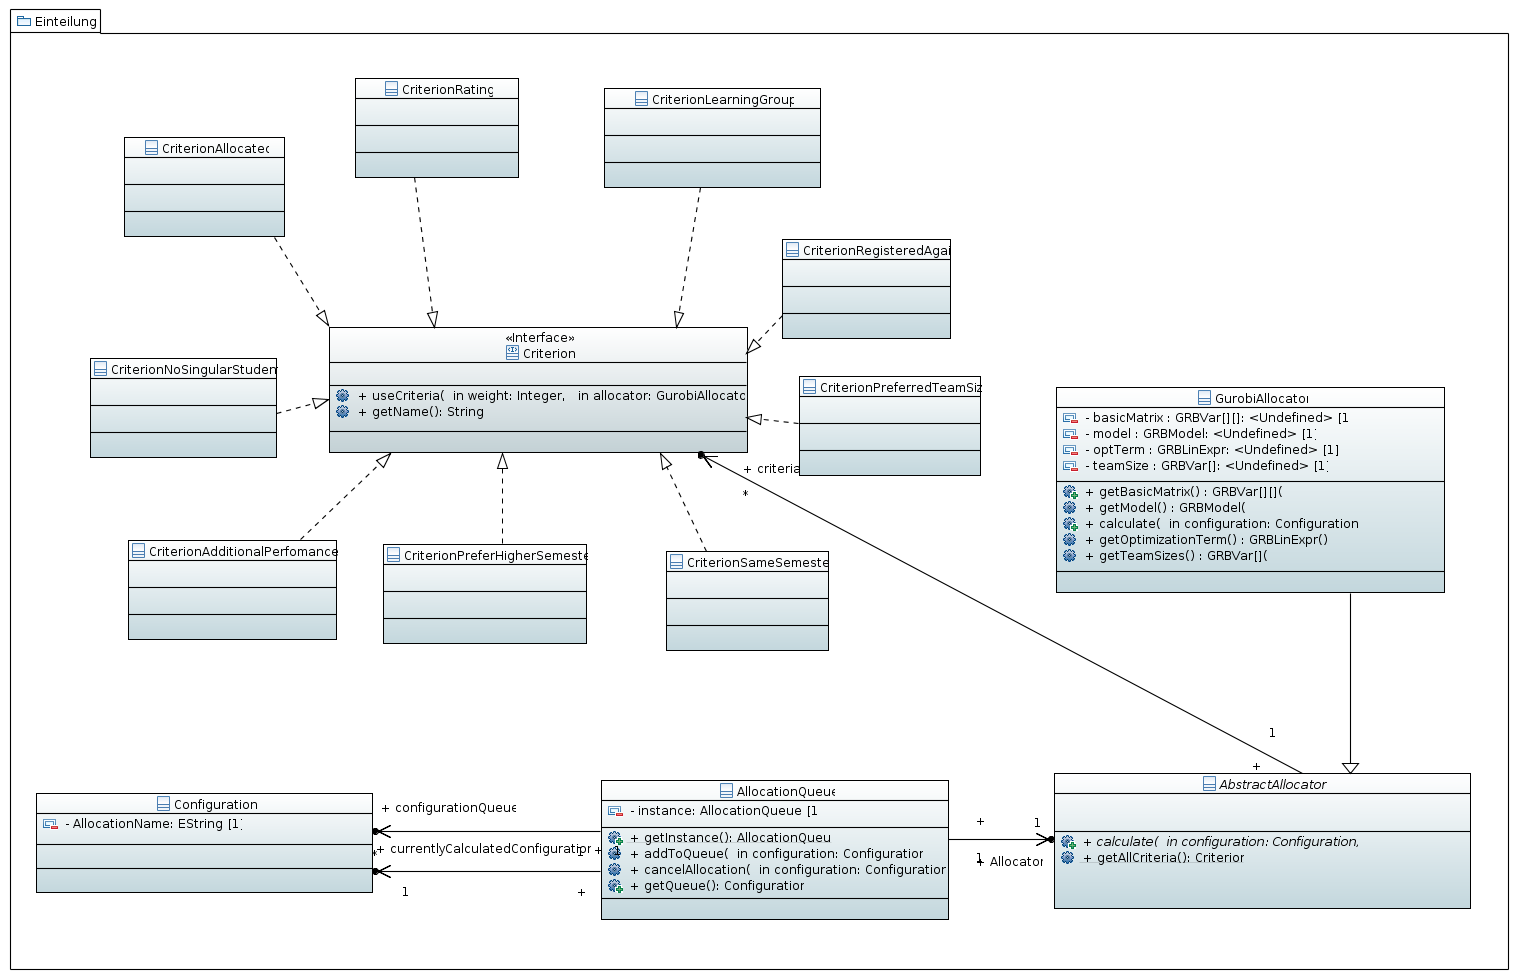
\includegraphics[width=\linewidth]{bilder/einteilung.png}
%TODO bild 
\end{frame}

\section{Sequenzdiagramm} %TODO gehört das zu einteilung?
\begin{frame}{Sequenzdiagramm}
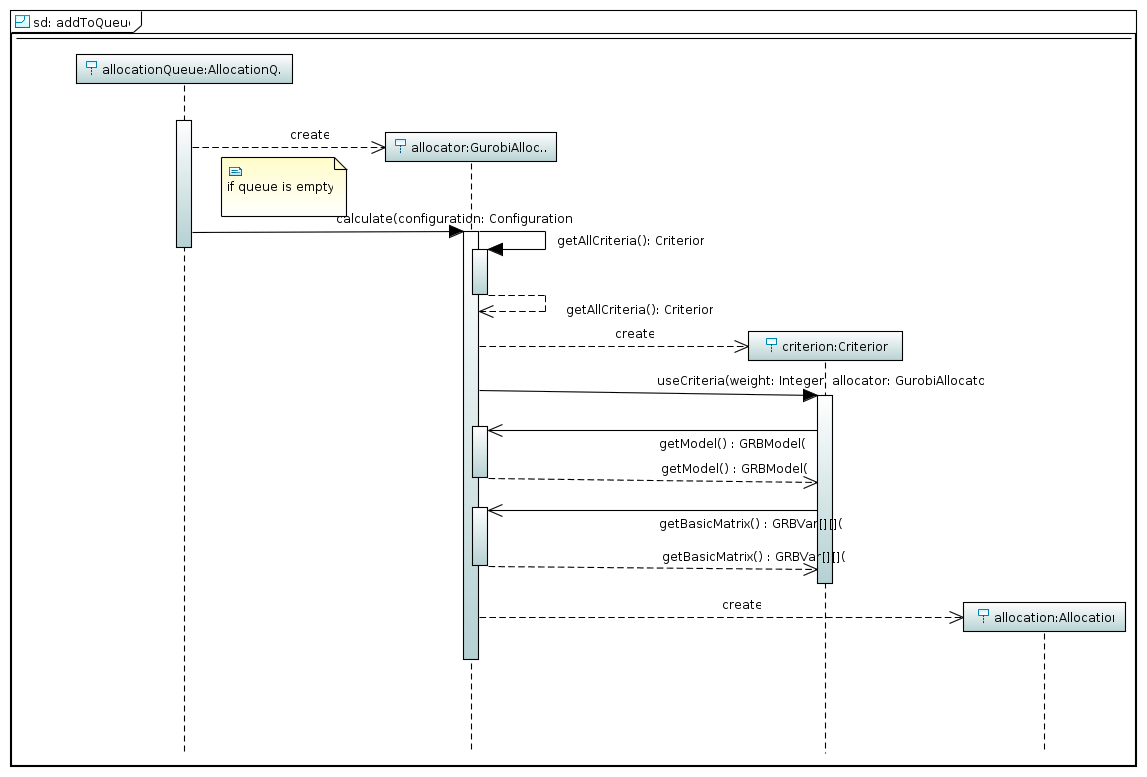
\includegraphics[width=\linewidth]{bilder/seqaddToQueue.png}
\end{frame}

\section{ILP}
\begin{frame}{ILP-Modell}
Aufteilung des ILP-Modells:
\begin{itemize}
  \item Basismodell
  \item Kriterien
\end{itemize}
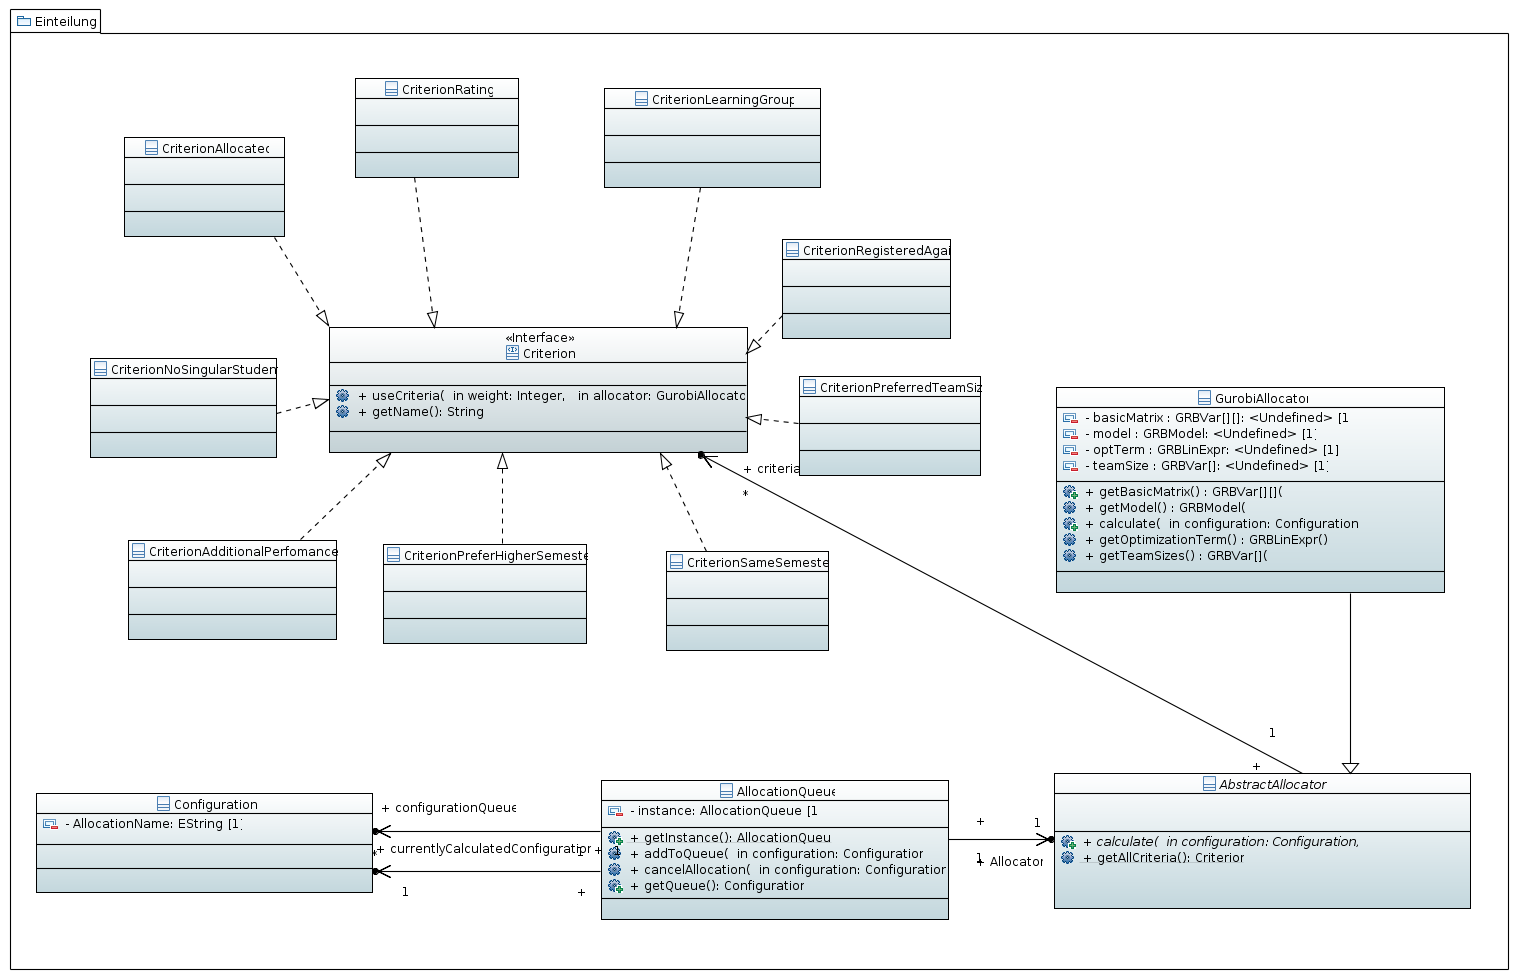
\includegraphics[width=\linewidth]{bilder/einteilung.png}
%TODO bild von UML
\end{frame}

\begin{frame}{Basismodell}
Das Basismodell besteht aus:
\begin{itemize}
  \item $N \times M$ Matrix - Student $n$ in Team $m$
  \item Basisconstraints 
  \item Optimierungsterm
  \item Hilfsvariablen
\end{itemize}
%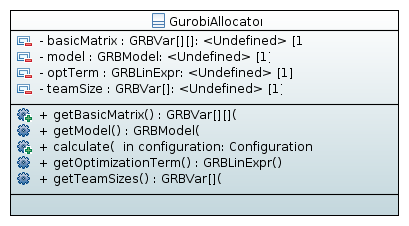
\includegraphics[width=\linewidth]{bilder/basismodell.png}
%TODO einen  basisconstraint?
\end{frame}

\begin{frame}{Kriterien}
\begin{itemize}
  \item Greifen auf Basismodell zu
  \item Erweitern Optimierungsterm und Constraints
  \item Sind über Serviceloader eingebunden
\end{itemize}
%TODO bild der Kriterien
\end{frame}

\begin{frame}{Beispielkriterium - Lerngruppen} %TODO welches? und bearbeiten
Jedes Paar Studierender $p:= (a,b)$ mit $a,b \in \{ 1\ldots N\}: a > b$
einer Lerngruppe das zusammenbleibt bekommt einen Bonus $LgBonus_l$ von
$\frac{10}{pair_l}$
\begin{align*}
\intertext{Als Constraints: }
0 &\le y_{lpt} \le 1  \\
y_{lpt} &= B(a,t) \wedge B(b,t)
%y_{lpt} \le B(k_1,t) + B(k_2,t) -1, \; y_{lpt} \le B(k_2,t), \; y_{lpt} \le
%B(k_2,t) 
\end{align*}
\begin{align*}
\intertext{Zum Optimierungsterm: } 
p_i \cdot LgBonus_l \cdot y_{lpt} \text{ für alle Paare, Lerngruppen und Teams}
\end{align*} 

\end{frame}

\appendix
\beginbackup

\begin{frame}{Fragen}
\printbibliography
\end{frame}

\backupend

\end{document}
